\documentclass{beamer}

\usepackage[orientation=landscape,size=a0,scale=1.4,debug]{beamerposter}
\mode<presentation>{\usetheme{mlr}}

\usepackage[sfdefault]{roboto}
\usepackage{roboto-mono}
\usepackage[T1]{fontenc}
\usepackage[utf8]{inputenc} % UTF-8
\usepackage[english]{babel} % Language
\usepackage{hyperref} % Hyperlinks
\usepackage{ragged2e} % Text position
\usepackage[export]{adjustbox} % Image position
\usepackage[most]{tcolorbox} % Code boxes
\usepackage{multido}

\hypersetup{
	hyperfootnotes=false,
	colorlinks=true,
	linktocpage=true,
	pdfauthor={mlr-org team},
	%linkcolor=[RGB]{3,99,142}, % mlr blue
	urlcolor=[RGB]{231,138,69}
}

\title{Hyperparameter Tuning with mlr3tuning :\,: CHEAT SHEET} % Package title in header, \, adds thin space between ::

\newlength{\columnheight} % Adjust depending on header height
\setlength{\columnheight}{84cm} 

\newtcolorbox{codebox}{%
	sharp corners,
	leftrule=0pt,
	rightrule=0pt,
	toprule=0pt,
	bottomrule=0pt,
	fontupper=\robotomono\small,
	hbox}

\newtcolorbox{codeboxmultiline}[1][]{%
	sharp corners,
	leftrule=0pt,
	rightrule=0pt,
	toprule=0pt,
	bottomrule=0pt,
	fontupper=\robotomono\small,
	#1}

\newtcolorbox{codeboxexample}{%
	sharp corners,
	leftrule=0pt,
	rightrule=0pt,
	toprule=0pt,
	bottomrule=0pt,
	fontupper=\robotomono\small,
	width=27cm,
	adjusted title=Example,
	fonttitle = \bfseries\Large,
	top = 0.5em}

\newtcolorbox{codeboxinline}{%
	sharp corners,
	leftrule=0pt,
	rightrule=0pt,
	toprule=0pt,
	bottomrule=0pt,
	hbox,
	nobeforeafter,
	fontupper=\robotomono\small,
	tcbox raise base}

\newcommand{\codeinline}[1]{\begin{codeboxinline}#1\end{codeboxinline}}
\newcommand{\sectionheading}[1]{{\color{mlrblue}\large\raggedright\textbf{#1}}\vspace{1em}}
\newcommand{\monospace}[1]{\multido{}{#1}{\space}}

\begin{document}
\begin{frame}[fragile]{}
	\begin{columns}
		\begin{column}{.245\textwidth}
			\begin{beamercolorbox}[center]{postercolumn}
				\begin{minipage}{.98\textwidth}
					\parbox[t][\columnheight]{\textwidth}{
						\begin{myblock}{Intro}
							\codeinline{TuningInstance} is evaluator 
							and container for resampled performances 
							of hyperparameter configurations of a learner 
							during tuning with a search algorithm. 
                            \codeinline{Tuner} generates candidate configurations 
                            and passes them to \codeinline{TuningInstance} 
                            until the budget of \codeinline{Terminator} is exhausted (5). 
							\vspace{1em}
							\\
                            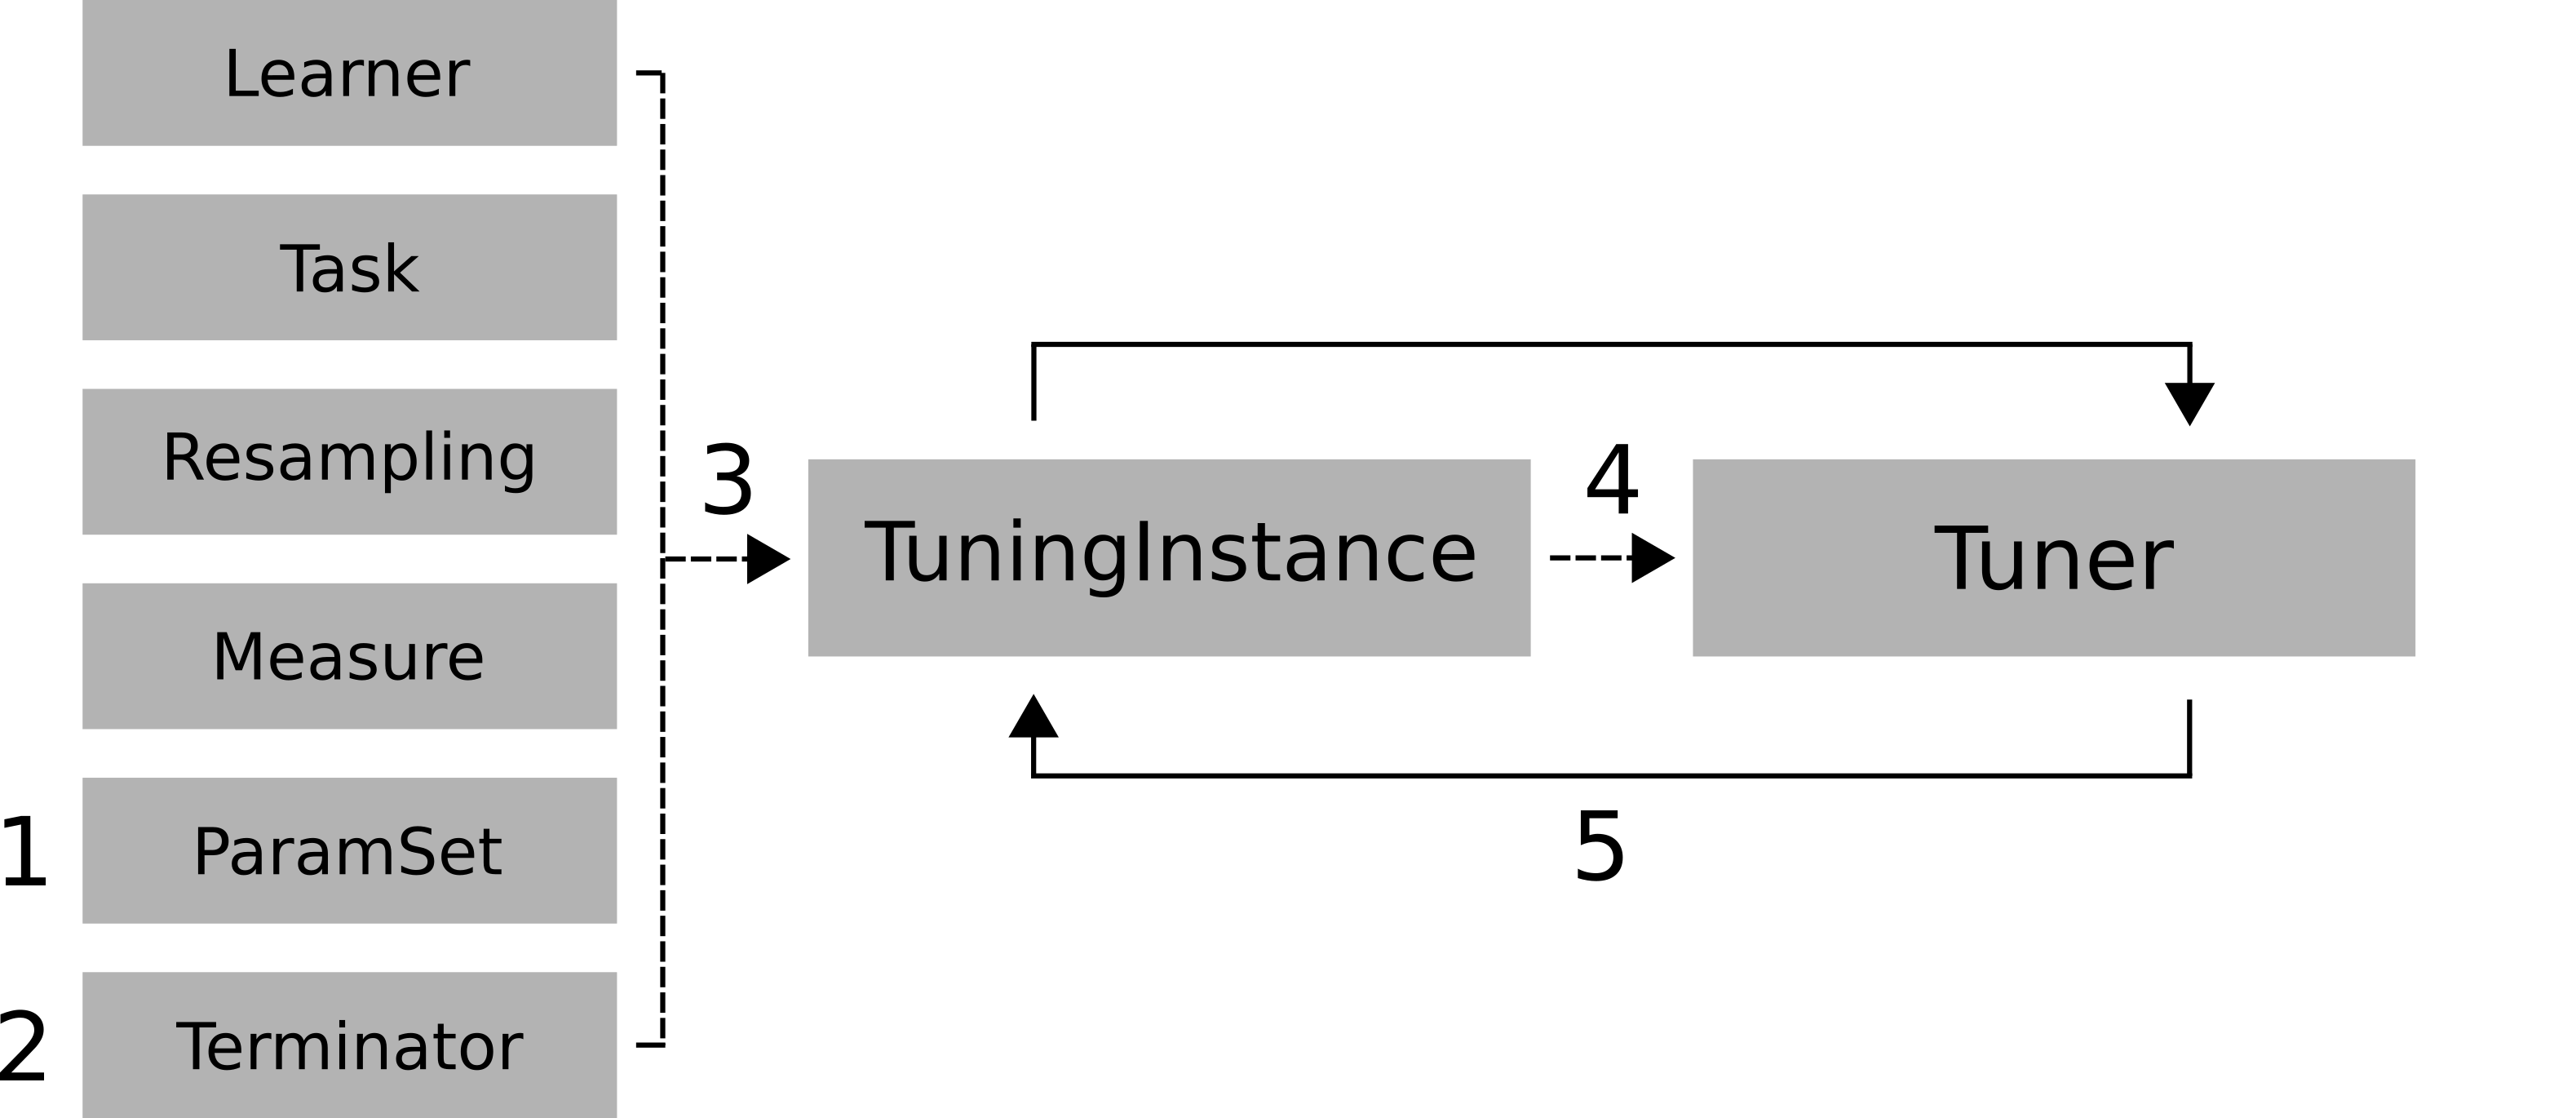
\includegraphics[width=\textwidth]{img/tuning_objects.png}
                            \\
                            \begin{codebox}
                            	{\scriptsize lgr::get\_logger("mlr3/mlr3tuning")\$set\_threshold(level)}
                            \end{codebox}
                            Change log-level only for mlr3tuning.
						\end{myblock}
						\begin{myblock}{ParamSet}
					        Hyperparameters and ranges for tuning (1). 
					        Scalar doubles, integers, factors, logicals are combined 
					        in a set to define the multivariate tuning space.
							\\
							\begin{codeboxmultiline}[width=20.75cm]
								tune\_ps = \textbf{ParamSet}\$new(list(\\
								\hspace*{1ex}\textbf{ParamInt}\$new(id, lower, upper),\\
								\hspace*{1ex}\textbf{ParamDbl}\$new(id, lower, upper),\\
								\hspace*{1ex}\textbf{ParamFct}\$new(id, levels),\\
								\hspace*{1ex}\textbf{ParamLgl}\$new(id)))
							\end{codeboxmultiline}
                            \codeinline{id} is param name in learner. 
                            \codeinline{lower}/\codeinline{upper} define 
                            numerical range, \codeinline{levels} for categories.
                            \vspace{1em}
                            \\ 
                            \sectionheading{Trafo  \& Dependencies}
							\begin{codeboxmultiline}[width=25.5cm]
								tune\_ps\$\textbf{trafo} = function(x, param\_set) \{\\
								\hspace*{1ex}x\$id = -log(x\$id); return(x)\}      
							\end{codeboxmultiline}
							Set a transformation for parameter \codeinline{id}. 
							The function transforms the hyperparameter configuration into another encoding 
							before passing them to the \codeinline{Learner}.
							\\
							\begin{codebox}
								tune\_ps\$\textbf{add\_dep}(id, on, cond)
							\end{codebox}
							Adds dependency to the \codeinline{ParamSet}, 
							so that \codeinline{id} depends on parameter \codeinline{on}.
							\codeinline{cond} is \codeinline{CondEqual\$new(rhs)} or \codeinline{CondAnyOf\$new(rhs)}.
						\end{myblock}
						\vfill}
				\end{minipage}
			\end{beamercolorbox}
		\end{column}
		\begin{column}{.245\textwidth}
			\begin{beamercolorbox}[center]{postercolumn}
				\begin{minipage}{.98\textwidth}
					\parbox[t][\columnheight]{\textwidth}{
						\begin{myblock}{Terminator Class}
							Stop criterion (2). Create with \codeinline{\textbf{term}(.key, ...)}
							\\
							\begin{itemize}
                                \item \codeinline{evals}
                                (\codeinline{n\_evals})\\
                                After a given amount of iterations.
								\item \codeinline{clock\_time} 
								(\codeinline{secs}, \codeinline{stop\_time})\\
								After a given absolute time.
								\item \codeinline{model\_time}
								(\codeinline{secs })\\
								After a given model time.
								\item \codeinline{perf\_reached}
								(\codeinline{level})\\
								After a specific numerical performance was reached.
								\item \codeinline{stagnation}
								(\codeinline{iters}, \codeinline{threshold})\\
								After the performance stagnates.
							\end{itemize}
							\vspace{1em}
							\begin{codebox}
								as.data.table(\textbf{mlr\_terminators})
							\end{codebox}
							Lists terminator dictionary.
							\\
							\begin{codebox}
								terminator = term("\textbf{combo}", terminators, any)
							\end{codebox}
							List of \codeinline{terminators} that terminate 
							if any (\codeinline{any = TRUE}) 
							or all (\codeinline{any = FALSE}) terminators are positive.
						\end{myblock}
						\begin{myblock}{TuningInstance Class}
							Defines search scenario (3). 
							Evaluates configurations proposed by \codeinline{Tuner} and stores results.
							\\
							\begin{codeboxmultiline}[width=23.7cm]
								instance = \textbf{TuningInstance}\$new(\\
								\hspace*{1ex}task, learner, resampling, measures,\\
								\hspace*{1ex}tune\_ps, terminator, bm\_args)
							\end{codeboxmultiline}
							\vspace{1em}
							\begin{codeboxexample}
								{\footnotesize
									tune\_ps = ParamSet\$new(list(\\
									\hspace*{1ex} ParamDbl\$new("C", lower = -5, upper = 5)))
									tune\_ps\$trafo = function(x, param\_set) \{\\
									\hspace*{1ex} x\$C = 2\textasciicircum x\$C\\
									\hspace*{1ex} x\}\\
									evals20 = term("evals", n\_evals = 20)
									\vspace{1em}
									\\
									instance = TuningInstance\$new(\\
									\hspace*{1ex} task, learner, resampling, measures,\\
									\hspace*{1ex} param\_set = tune\_ps, terminator = evals20,\\
									\hspace*{1ex} bm\_args = list(store\_models = TRUE))\\
									tuner = tnr("grid\_search", resolution = 5)
									\vspace{1em}
									\\
									tuner\$tune(instance)\\
									instance\$result}
							\end{codeboxexample}
						\end{myblock}
						\vfill}
				\end{minipage}
			\end{beamercolorbox}
		\end{column}
		\begin{column}{.245\textwidth}
			\begin{beamercolorbox}[center]{postercolumn}
				\begin{minipage}{.98\textwidth}
					\parbox[t][\columnheight]{\textwidth}{
						\begin{myblock}{Tuner Class}
                            Tuning strategy. Create witth \codeinline{\textbf{tnr}(.key, ...)}
							\\
							\begin{itemize}
								\item \codeinline{grid\_search}
								(\codeinline{resolution}, \codeinline{batch\_size})\\
								Grid search.
								\item \codeinline{random\_search}
								(\codeinline{batch\_size})\\
								Random search.
								\item \codeinline{gensa}
								(\codeinline{smooth}, \codeinline{temperature})\\
								Generalized simulated annealing.
								\item \codeinline{design\_points}
								(\codeinline{batch\_size }, \codeinline{design})\\
								All points user-specified.
							\end{itemize}
							\vspace{1em}
							\begin{codebox}
								as.data.table(\textbf{mlr\_tuners})
							\end{codebox}
							Lists tuner dictionary.
						\end{myblock}
						\begin{myblock}{Starting the Tuning}
							\begin{codebox}
								tuner\$\textbf{tune}(instance)
							\end{codebox}
							Starts the tuning (4).
							\\
							\begin{codebox}
								instance\$\textbf{archive}(unnest)
							\end{codebox}
							Returns all tried configurations and their resampling results. 
							Use \codeinline{unnest} to display hyperparameters without
							(\codeinline{tune\_x}) or with (\codeinline{params}) trafo applied.
							\\
							\begin{codeboxmultiline}[width=27cm]
								{\tiny
									instance\$archive()\\
									\#\# nr batch\_nr ... resample\_result\monospace{2}iters params tune\_x classif.ce\\
									\#\#\monospace{2}1\monospace{8}1 ...\monospace{1}<ResampleResult> 
									\monospace{4}5 <list> <list>\monospace{2}0.2825482\\
									\#\#\monospace{2}2\monospace{8}1 ...\monospace{1}<ResampleResult>
									\monospace{4}5 <list> <list>\monospace{2}0.2825482\\
									\#\#\monospace{2}3\monospace{8}2 ...\monospace{1}<ResampleResult>
									\monospace{4}5 <list> <list>\monospace{2}0.2696206\\
									\#\#\monospace{2}4\monospace{8}2 ...\monospace{1}<ResampleResult>
									\monospace{4}5 <list> <list>\monospace{2}0.2721586}
							\end{codeboxmultiline}
							\vspace{1em}
							\begin{codebox}
								instance\$\textbf{result}
							\end{codebox}
							Returns list with optimal configuration and estimated performance.
							\\
							\begin{codebox}
								{\footnotesize learner\$param\_set\$values = instance\$result\$params}
							\end{codebox}
							Set optimized hyperparameters in \codeinline{Learner}.
							\\
							\begin{codebox}
								future::\textbf{plan}(strategy)
							\end{codebox}
							Speed up tuning by using future backend.
						\end{myblock}
						\vfill}
				\end{minipage}
			\end{beamercolorbox}
		\end{column}
		\begin{column}{.245\textwidth}
			\begin{beamercolorbox}[center]{postercolumn}
				\begin{minipage}{.98\textwidth}
					\parbox[t][\columnheight]{\textwidth}{
						\begin{myblock}{AutoTuner Class}
							Wraps learner and adds automatic tuning. 
							\\
							\begin{codeboxmultiline}[width=20cm]
								at = \textbf{AutoTuner}\$new(\\
								\hspace*{1ex}learner, resampling, measures, \\
								\hspace*{1ex}tune\_ps, terminator, tuner)
							\end{codeboxmultiline}
							\vspace{1em}
                            Inherits from \codeinline{Learner} class; can be used like it. 
                            Training starts tuning on the training set,
                            and after completion trains the learner finally with 
                            this the optimal configuration on the full training set.
							\begin{codeboxmultiline}[width=16.5cm]
								at\$\textbf{train}(task)\\
								at\$\textbf{predict}(task, row\_ids)
							\end{codeboxmultiline}
						\end{myblock}
						\begin{myblock}{Nested Resampling}
							Resampling the \codeinline{AutoTuner} achieves nested resampling 
							with an inner and outer loop. 
							\\
							\begin{codeboxexample}
								{\scriptsize
									resampling\_inner = rsmp("holdout")
									\vspace{1em}
									\\
									at = AutoTuner\$new(learner, resampling\_inner, \\
									\hspace*{1ex}measures, tune\_ps, evals20, tuner) \\
									at\$store\_tuning\_instance = TRUE
									\vspace{1em}
									\\
									resampling\_outer = rsmp("cv", folds = 2)\\
									rr = resample(task, at, resampling\_outer, \\
									\hspace*{1ex}store\_models = TRUE)
									\vspace{1em}
									\\
									rr\$data\\
									\#\# ...\monospace{3}learner\monospace{5}resampling iteration
									prediction\\
									\#\# ... <AutoTuner> <ResamplingCV>\monospace{9}1\monospace{5}<list>\\
									\#\# ... <AutoTuner> <ResamplingCV>\monospace{9}2\monospace{5}<list>}
							\end{codeboxexample}
							\vspace{1em}
							\begin{codebox}
								rr\$\textbf{aggregate()}
							\end{codebox}
							Aggregates performance of outer results.
							\\
							\begin{codebox}
								rr\$data\$learner[[1]]\$\textbf{tuning\_result}
							\end{codebox}
							Retrieve inner tuning results.
						\end{myblock}
						\vfill}
				\end{minipage}
			\end{beamercolorbox}
		\end{column}
	\end{columns}
\end{frame}
\end{document}
